\chapter{Evaluation}
\label{chapter6}
Um die Praxistauglichkeit zu überprüfen, werden nun ausgewählte Daten
mithilfe des entwickelten Tools evaluiert.
Zur Bewertung des Clusterings unterscheidet man \emph{externe}
und \emph{interne} Indizes \citep{aghabozorgi_time-series_2015, warren_liao_clustering_2005}.
Bei einem \emph{externen Index} werden Ground-Truth-Daten extern bereitgestellt.
Nach dem Clustering kann der Grad der Übereinstimmung zwischen gefundenen Cluster
und den vorgegebenen Clustern überprüft werden.
Bei \emph{internen Indizes} müssen Qualität der Cluster hingegen
ohne zusätzliche Informationen überprüft werden \citep{aghabozorgi_time-series_2015, warren_liao_clustering_2005}.
Dazu soll in \autoref{6-Statistical} die Standardabweichung genutzt werden,
um ein Maß für die Ähnlichkeit von Clustern-Komponenten zu erhalten.
Dabei sollte die Übereinstimmung bei Records des selben Clusters hoch
und bei Records verschiedener Cluster niedrig sein \citep{aghabozorgi_time-series_2015}.

\section{Einführende Bemerkungen}
\label{6-Bemerkungen}
Statt den gesamten in \autoref{2-StrukturDatensatz} beschriebenen Datensatz zu verwenden
sollen geeignete Teilmengen genutzt werden.
Zudem wurden die Daten gefiltert bereitgestellt.
Zu kurze oder fehlerhafte Records wurden aussortiert.
Außerdem wurden der Datensatz nach Personenzahl sortiert.
Das Filtern der Daten gehört nicht zu den Anforderungen an das entwickelte Tool
und wird daher nicht in dieser Arbeit betrachtet.
Dennoch sollte dem Nutzer bewusst sein,
dass damit aussagekräftigere Ergebnisse erzielbar sind.
Gerade die separate Betrachtung von Records nach Personenzahl kann helfen,
wiederkehrende Bewegungsmuster durch Clustering zu erkennen.
Die Anzahl gibt dabei immer an wie viele Personen sich maximal
zu einem Zeitpunkt in der Aufnahme befinden.
In \autoref{6-GroundTruth} und \autoref{6-Statistical} werden nur Records mit ein bis drei Personen betrachtet.

Ebenfalls zu erwähnen, ist die Bedeutung eines geeigneten Threshold-Wertes für ein erfolgreiches Clustering.
Dieser kann je nach vorliegenden Daten, verwendeten Attributen und Zielstellung variieren.
Häufig ist daher ein {\glqq Herantasten\grqq} nötig.
Abhängig davon wie viele Cluster am Ende erwünscht sind
und wie stark die Cluster-Komponenten voneinander abweichen dürfen,
muss ein anderer Wert gewählt werden.

\section{Ground-Truth Analyse}
\label{6-GroundTruth}
Für die Ground-Truth Analyse wurden für die Fälle eine bis drei Personen jeweils zufällig 25 Records gewählt.
Diese wurden mithilfe des Visualizers und Kinect Studio visualisiert und manuell in Cluster eingeteilt.
\autoref{fig:Clusters} zeigt jeweils die Visualisierung eines Repräsentanten der Cluster.
\begin{figure}[ht]
    \begin{center}
    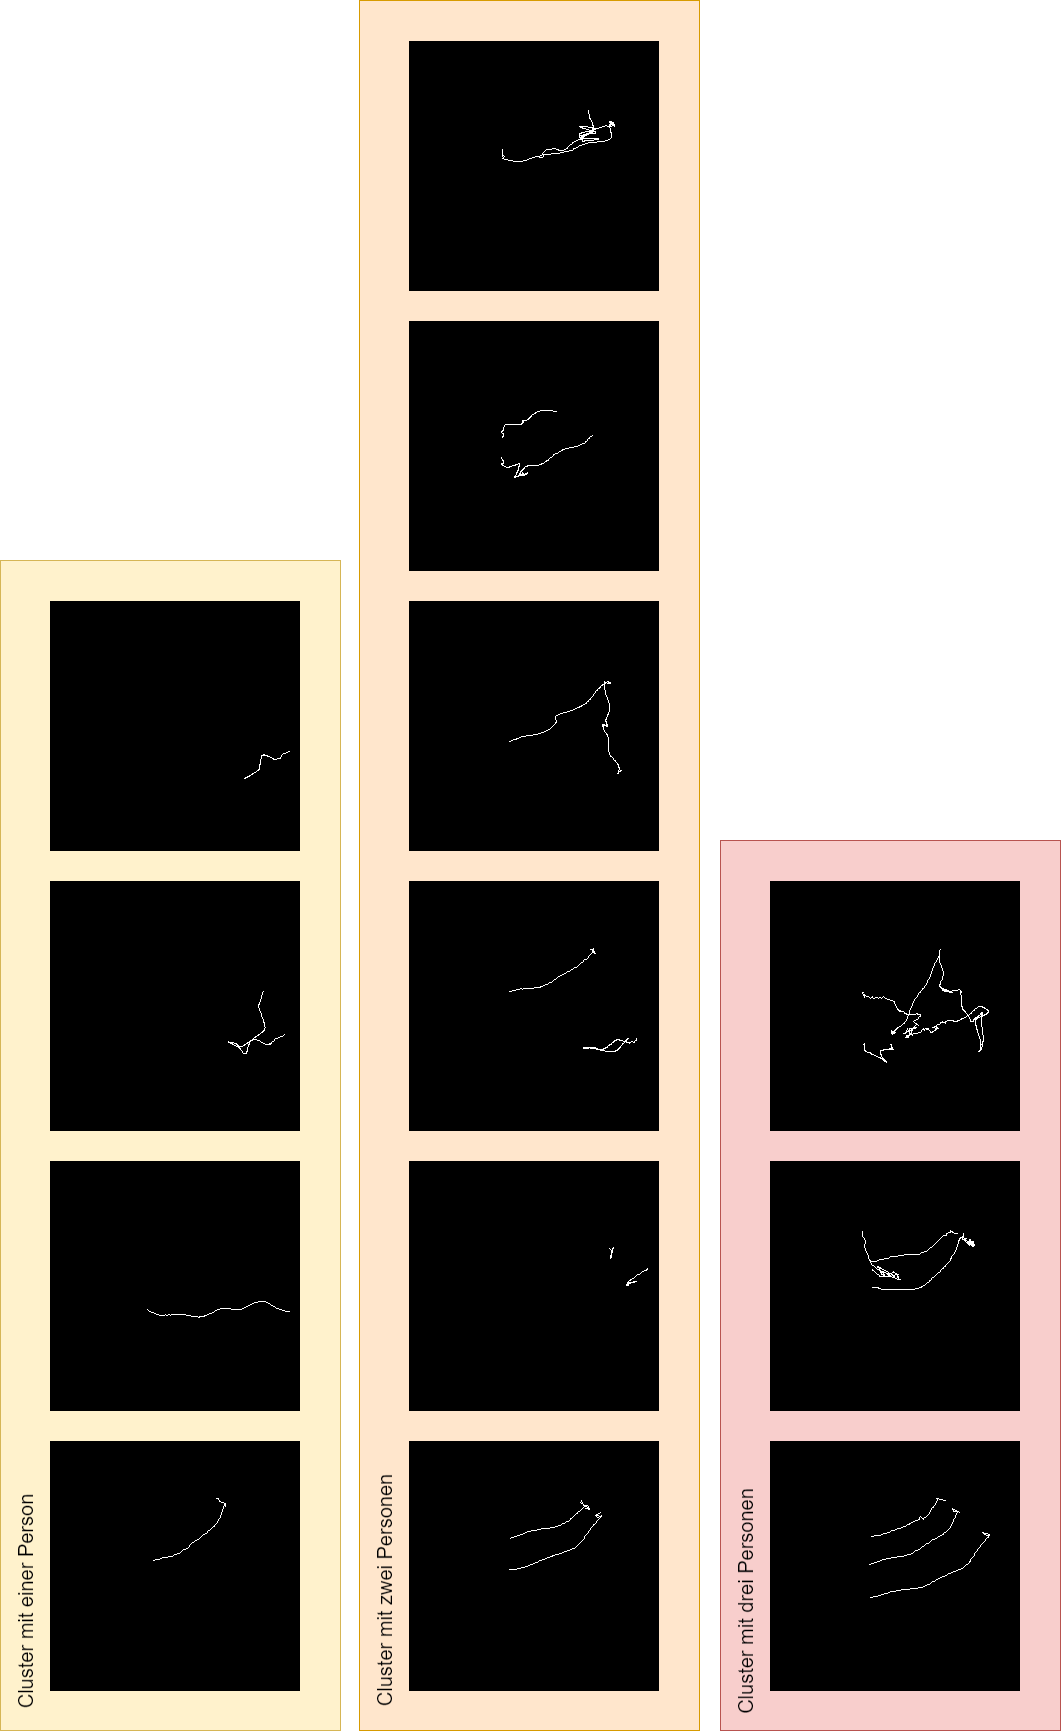
\includegraphics[width=0.8\textwidth]{clusters.png}
    \end{center}
    \caption{Repräsentanten der manuell erstellten Cluster.}
    \label{fig:Clusters}
\end{figure}
Die Ergebnisse und eine sprachliche Beschreibung des Inhalts
können jeweils im \emph{resources}-Verzeichnis des Projektordners eingesehen werden.
Anschließend wurde das hierarchische Clustering gestartet.
Der Threshold wurde dabei jeweils so gewählt,
dass genau so viele Cluster entstehen wie manuell erkannt wurden.
Die Auswertung zeigt, dass die vom Tool berechneten Cluster genau mit den Ground-Truth Daten übereinstimmen.

\section{Statistische Analyse}
\label{6-Statistical}